\include{abntex2-modelo-include-comandos}

\chapter{Referencial teórico}\label{cap_trabalho_academico}

Como mencionado no capítulo anterior, a criação da plataforma é baseado em diversas tecnologias e conceitos que asseguram a segurança de um sistema descentralizado.

Dessa forma, nesse capítulo será abordado os pontos essenciais para entender a criação do projeto, tais como: o que é um Freelancer e uma plataforma de Freelance, sistemas centralizados e descentralizados, \textit{Ethereum} e redes similares, a importância do \textit{Bitcoin} como um sistema de pagamento, entre outros tópicos.

\section{Contexto}

Antes de entrar em conceitos fundamentais, é necessário entender sobre o que se trata o projeto, ou seja, entender o que é um Freelancer, o que são plataformas de Freelance e quais são as plataformas que existem hoje.

\subsection{Freelancer}

\textit{Freelancers} são pessoas autônomas que têm uma associação de curto prazo baseada em tarefas com o empregador e, não são empregados da empresa. A sua associação com a empresa é apenas até que a tarefa atribuída seja concluída com sucesso.\cite{freelance}

Eles tem a obrigação de completar a tarefa com alta qualidade dentro do prazo acordado em troca de dinheiro (previamente acordado com o empregador). Durante o tempo que o freelancer estiver realizando a tarefa, ele fica livre para realizar acordo com diversos empregadores, resumindo, os \textit{freelancers} realizam vários projetos em paralelo.

\subsection{Plataformas de Freelance}
Plataformas \textit{freelancer} têm mantido perfis de trabalho dos \textit{freelancers} e empregadores para ajuda-los a estabelecer confiança mútua, servindo como uma ponte de ligação entre os dois perfis. Além disso, os empregadores depositam o valor do serviço do freelance para a plataforma, que só libera o valor para o freelance depois da entrega do serviço ser validada pelo empregador.\cite{freelance}

À medida que a cultura de \textit{freelancer} ficou famosa durante todos esses anos, centenas de sites foram lançados que fornecem serviços \textit{freelancer}. Entre os mais famosos da internet podemos citar \textit{Upwork}, \textit{People Per Hour} e \textit{Fiverr} e no Brasil, \textit{Workana} \cite{the_freelancer}.

\subsubsection{Workana}

\textit{Workana} é uma plataforma de mercado para trabalho \textit{freelancer} e remoto, de contratação de trabalhadores independentes. A empresa tem sua sede na Argentina e possui escritórios no Brasil, na Colômbia e no México, a plataforma está disponível em espanhol, inglês e português. \cite{workana}

Ao usar o \textit{Workana} como empregador você pode: publicar um projeto para começar a receber propostas, pode interagir e selecionar o melhor \textit{freelancer}, e por fim, realizar o pagamento do trabalho realizado para o \textit{freelancer}. E como \textit{freelancer}, você pode encontrar projetos, enviar propostas para os clientes e trabalhar com total autonomia. \cite{workana}

\subsubsection{Upwork}

\textit{Upwork}, anteriormente \textit{Elance-oDesk}, é uma plataforma americana de \textit{freelancers} atualmente com sede em Santa Clara e São Francisco, Califórnia. Em 2017, \textit{Upwork} tinha mais de 12 milhões de \textit{freelancers} registrados e 5 milhões de clientes. Em março de 2022, a \textit{Upwork} foi nomeada para a lista das 100 empresas mais influentes do ano de 2022 da \textit{TIME}. \cite{upwork}

Assim como a \textit{Workana}, é possível criar projetos, selecionar \textit{freelancers}, realizar pagamentos do trabalhos contratados e receber por esses trabalhos realizados como \textit{freelancer}.

\section{Conceitos Fundamentais}

Abaixo, será falado um pouco dos conceitos fundamentais que irá ser o pilar das tecnologias e ferramentas apresentadas posteriormente no trabalho. E partir desses conceitos, será possível entender como a \textit{Blockchain} e \textit{Bitcoin} funcionam, dessa forma, entender também o por que dessas tecnologias terem sido escolhidas para desenvolver a plataforma.

\subsection{Sistemas Centralizados}

Um sistema centralizado pode ser descrito como uma arquitetura de cliente e servidor, no qual o cliente realiza requisições e o servidor responde as requisições recebidas de um cliente. E esse sistema, no começo da Word Wide Web, se tornou muito popular através dos protocolos como: \textit{File Transfer Protocol} (FTP), \textit{Simple Mail Transfer Protocol} (SMTP)
e \textit{Hypertext Transfer Protocol} (HTTP). \cite{client_server_model}

\begin{figure}[h!]
  \centering
  \caption{Arquitetura Cliente/Servidor}
  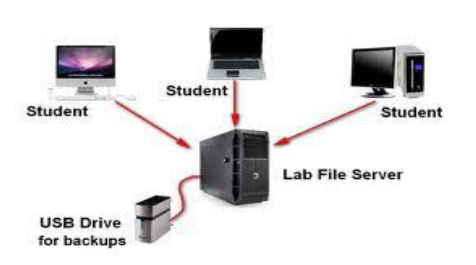
\includegraphics[width=300px]{src/images/client-server.png}
  \subcaption{Fonte: \cite{client_server_model} }
  \label{fig:client_server_fig}
\end{figure}

Para \citeauthor{held2000server}, um computador, notebook ou dispositivo é representação de um cliente, e junto de um servidor, possuem uma relação de cooperação para executar uma ação iniciada pelo cliente final que retornará algum recurso ou modificará algum estado dentro do servidor. A representação dos diversos clientes conectando em um único servidor é descrito na Figura \ref{fig:client_server_fig}.

\subsection{Sistemas Descentralizados}

De acordo com \cite{distributed}, um sistema descentralizado, ou um sistema distribuído, é a composição de diversos computadores que forma um sistema que se comunica em uma rede de computadores, de forma que, através de protocolos como \textit{HTTP}, \textit{SMTP}, etc... permitem a execução de atividades de forma distribuída.

\cite[p.17]{design_distributed_systems} diz que "devido à sua natureza distribuída, quando estruturados adequadamente, os sistemas distribuídos são inerentemente mais confiáveis". Diferente do modelo de cliente-servidor, a mesma tarefa pode ser executada em diversos computadores, de forma que, se ocorrer uma falha em computador, o sistema ainda continua operando por que a tarefa pode ser processada por qualquer computador conectado no sistema.

Além da confiabilidade e da disponibilidade, em um âmbito mais amplo, \citeauthor{decentralization} descreve que a descentralização pode ser usada para construir uma estrutura de governança que permita diversos grupos viverem de forma pacífica. Isso ocorre porque uma estrutura descentralizada não é baseada em confiança em uma autoridade central, ao contrário disso, ela delega poder a autoridades menores para ter mais efetividade e segurança ao não ter um ponto central de falha.

\section{Tecnologias}

Nesta seção, será falado sobre as tecnologias que compõem a plataforma e porque elas foram construídas, de forma que, exemplifique a sua importância na criação da plataforma.

\subsection{Blockchain}

O \textit{Blockchain} é uma tecnologia para armazenar as informações de forma segura e imutável através do que ela chama de blocos. Os blocos são um recipiente onde é agrupado diversas transações e, após uma certa quantidade de transações, um bloco é finalizado e outro bloco é criado, ao mesmo tempo, uma assinatura digital chamado de \textit{Hash} é criado associando o bloco anterior com o novo bloco, como pode ser visto na Figura \ref{fig:blockchain_structure} \cite{blockchain}.

\begin{figure}[h!]
  \centering
  \caption{Representação da estrutura do Blockchain.}
  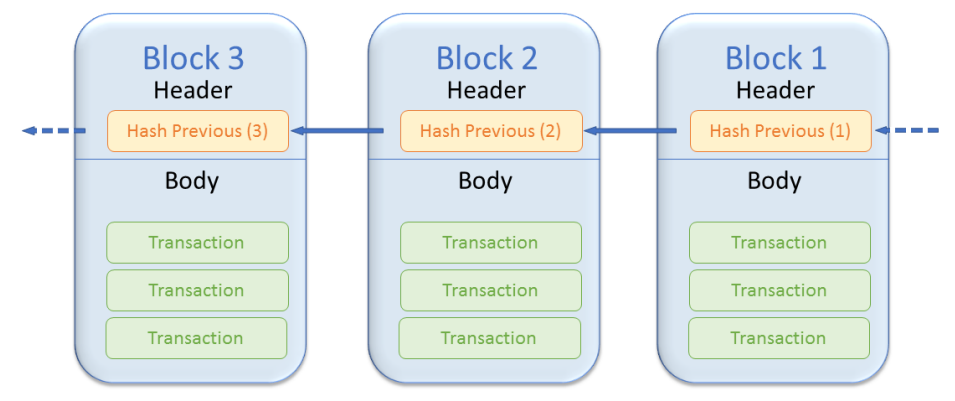
\includegraphics[width=300px]{src/images/representacao_blocos_blockchain.png}
  \subcaption{Fonte: \cite{blockchain_ref_for_block_explanation}}
  \label{fig:blockchain_structure}
\end{figure}

Ao associar um bloco ao anterior, se um participante malicioso deseja alterar o conteúdo de um bloco passado, ele necessariamente irá alterar o \textit{Hash} desse mesmo bloco, porque o \textit{Hash} é gerado baseado no conteúdo do bloco. Ao modificar o \textit{Hash}, qualquer bloco que foi gerado posteriormente, e que estava conectado a esse bloco modificado, se tornará inválido. Isso acontece por que os blocos posteriores não vão possuir o novo \textit{Hash}, e dessa forma, para detectar um bloco modificado só seria necessário comparar o \textit{Hash} do bloco atual e o \textit{Hash} no bloco posterior \cite{blockchain_ref_for_block_explanation}. 

Dessa forma, ao usar a estrutura do \textit{Blockchain}, é possível criar uma rede onde qualquer pessoa pode participar ao possuir uma cópia do histórico de transações, reduzindo a necessidade de confiança entre as partes e aumentando a transparência ao permitir que qualquer pessoa possa auditar as transações armazenadas \cite{blockchain}.

Contudo, para coordenar todos os participantes da rede, é necessário que haja algum algoritmo de consenso de forma a suportar as falhas bizantinas, que é quando a falha de um nó faz com que o sistema como um todo fique comprometido \cite{byzantine_fault_tolerance}. Na seção a seguir, será explicado os algoritmos de consenso e também como o \textit{Bitcoin} propôs uma solução para esse problema.

\subsection{Bitcoin}

Segundo \cite{bitcoin2}, \textit{Bitcoin} é um sistema descentralizado de dinheiro eletrônico \textit{Peer-to-Peer} (P2P) sem um servidor central ou partes confiáveis. Os usuários têm as chaves criptográficas para o seu próprio dinheiro e transacionam diretamente na rede com outros usuários do sistema.

Em poucas palavras, o \textit{Bitcoin} é uma forma de dinheiro, assim como o real, o dólar ou o euro, com a diferença de ser puramente digital e não ser emitido por nenhum governo. O seu valor é determinado livremente pelos indivíduos no mercado. Para transações online, é a forma ideal de pagamento, pois é rápido, barato e seguro.

Além disso, para resolver o problema de gasto-duplo, assim como as falhas de Bizantino, o \textit{Bitcoin} utiliza o algoritmo de consenso chamado \textit{Proof-of-Work} (Prova de Trabalho). A ideia inicial desse tipo de técnica para solucionar o problema foi introduzido por \cite{pricing_via_processing}, onde descrito uma função que necessitasse de um custo computacional relevante para escrever uma mensagem, ao mesmo tempo em que, fosse barato para verificar se essa mensagem era verdadeira.

E alguns anos mais tarde, \cite{proofs_of_work_original} trouxe a ideia do protocolo chamado de \textit{Proof-of-Work}, ou prova de trabalho. \citeauthor{proofs_of_work_original} o descrevia como "um protocolo no qual um provador demonstra a um verificador que ele gastou um certo nível de esforço computacional em um intervalo de tempo especificado". 

Dessa forma, \citeauthor{bitcoin} utilizou esse protocolo e o montou da seguinte maneira: é necessário que o bloco submetido na rede possua uma prova de trabalho, isso garante que, para fraudar a rede, seja necessário ter mais de 51\% do poder computacional porque só dessa forma seria possível ultrapassar a velocidade de outros nós e convencer que a sua versão é a correta. Além disso, a dificuldade dessa prova de trabalho é constantemente reajustada, com o objetivo de manter um tempo médio de criação de um novo bloco em torno de 10 minutos, isso ajuda a evitar que um novo modelo de computador quebre o equilíbrio da rede.

\subsection{Ethereum}

Assim como o \textit{Bitcoin}, o \textit{Ethereum} é um sistema descentralizado de dinheiro eletrônico e também pode ser descrito por \cite{ethereum2}, como uma rede de criptomoedas popular que pode suportar DApps.

No começo do desenvolvimento do trabalho, a \textit{Ethereum} possuía um modelo de consentimento baseado em \textit{Proof-of-Work}, contudo, ouve uma migração para o tipo de consentimento chamado \textit{Proof-of-Stake} com o objetivo de diminuir as taxas de transação e o consumo de energia.

A ideia por trás do \textit{Proof-of-Stake} é fornecer proteção contra o ataque de fraude ao possuir 51\% da rede, além de permitir uma capacidade maior de transações por segundo e também reduzir custos de taxa de transação. Como \cite{larimer2013transactions} descreve, a ideia é ter nós responsáveis por dizer se um bloco é válido ou não, e em essência, toda rede é em partes um \textit{Proof-of-Stake} porque há nós com direito de decidir se um bloco é válido ou não. 

Contudo, na \textit{Ethereum}, o que dá esse direito é o depósito que o dono do nó faz antecipadamente. Esse depósito tem o objetivo de garantir e assegurar que o dono do nó não vá querer cometer alguma fraude, e caso uma fraude venha a ocorrer por aquele nó, o dinheiro depositado é totalmente perdido. Porém, ao utilizar esse tipo de consenso, a segurança como um todo é diminuída porque é necessário a coordenação de menos nós para que ocorra uma fraude na rede. 

\subsection{Peer-to-Peer}

\textit{Peer-to-Peer} refere-se a troca direta de algum ativo, como uma moeda digital, entre partes individuais sem o envolvimento de uma autoridade central. Uma troca de moeda estritamente \textit{peer-to-peer} foi o principal objetivo que impulsionou a criação do \textit{Bitcoin}. \cite{peer-to-peer}

\subsection{Smart Contracts}

\textit{Smart Contracts}, traduzido como Contratos Inteligentes, são scripts auto-executáveis que residem em \textit{blockchain}, tem como objetivo permitir adequação, distribuição e automatização de fluxos de trabalho. \cite{smart_contract2}

É definida por \citeauthor{smart_contract} como “um protocolo de transação computadorizado que executa os termos de um contrato". Os contratos inteligentes nos permitem que cálculos de propósito geral ocorram na cadeia. No entanto, eles se destacam quando são encarregados de gerenciar interações orientadas por dados entre entidades da rede.

\subsection{DApps}

Um aplicativo descentralizado (\textit{DApp}) é um aplicativo construído em uma rede descentralizada que combina um contrato inteligente e uma interface de usuário front-end sendo executado em uma rede \textit{Peer-to-Peer}. No \textit{Ethereum}, os contratos inteligentes são acessíveis e transparentes – como \textit{APIs} abertas – para que seu \textit{DApp} possa até incluir um contrato inteligente que outra pessoa tenha escrito.\cite{DApps}

\section{Resolução de Conflitos}

Nesta seção, será falado sobre os aspectos da resolução de conflitos, uma vez que as duas partes podem ter um desacordo um com o outro, como a plataforma lidará para resolver esse conflito. Para chegar em uma solução, será descrito primeiro o que será considerado um conflito e quais as formas que a academia encontrou de resolver, e qual é a forma que foi escolhida.

\subsection{Definição de conflito}

Para \cite[p.18]{rahim2017managing}, o conflito é "um processo interativo manifestado em incompatibilidade, desacordo ou dissonância dentro ou entre entidades sociais". Ao aplicar o contexto de uma interação entre duas pessoas no qual uma deseja contratar a outra, um conflito pode surgir quando, por exemplo, a parte contratante acha que o que foi entregue não é suficiente e o contratado acredita que deve receber pelo serviço prestado.

Já \cite{nicholson1992rationality} define que é uma atividade entre seres conscientes, que não necessariamente são racionais, além disso, é necessário ter termos, necessidades ou obrigações entre as partes envolvidas. Ao estender, (\citeauthor{nicholson1992rationality}) também completa que um conflito pode existir quando duas pessoas querem realizar ações que são mutuamente incompatíveis.

Para ambos os autores, o que define o conflito é o desacordo e as ações mutuamente incompatíveis, e alinhado ao exemplo do contrante e o contratado, temos que um conflito é algo comum e que precisa ser tomado ações pacíficas entre ambas as partes para ser resolvido, e é sobre isso que tratará a próxima seção.

\subsection{Formas de Resolução de Conflito}

Em seu livro, \cite{bercovitch2019social} menciona três formas básicas de resolução de conflito:

\begin{itemize}
\item Com coerção ou violência.
\item Com negociação ou barganha.
\item Ou com uma intervenção de um terceiro.
\end{itemize}

Se tratando de uma sociedade onde violência é inaceitável, a primeira opção está fora de cogitação para a plataforma porque o intuito é fornecer segurança e confiabilidade aos usuários da plataforma.

Sobre a negociação, \cite[p.3]{behavioral_theory_of_labor_negotations} sugeria que negociação era "uma interação deliberada de duas ou mais unidades sociais complexas que estão tentando definir ou redefinir os termos de sua interdependência". Quanto a barganha, \cite{nicholson1992rationality} descrevia a barganha como um conflito parcial de objetivos no qual as partes se esforçam para encontrar um acordo mutuamente satisfatório. Dessa forma, a plataforma em si não precisa fazer nada proativamente em busca de resolver esse conflito, visto que, tanto na negociação quanto na barganha, é necessário apenas o envolvimento das partes interessadas e que o conflito não seja completamente irreconciliável.

Contudo, em um caso onde o conflito chegue ao ponto de ser irreconciliável, é possível optar para a terceira forma de resolução de conflito, a intervenção de um terceiro, no qual será falado em mais detalhes na próxima seção.

\subsection{Intervenção de Terceiros}

Quando se faz necessário a intervenção de um terceiro para a resolução de um conflito, o que antes era uma díade acaba se tornando uma tríade, e dessa forma, esse terceiro agente tem o poder de afetar os resultados e o comportamentos das partes envolvidas \cite{bercovitch2019social}.

Além disso, \citeauthor{bercovitch2019social} diz que esse tipo de resolução de conflito ocorre quando o conflito se estende por muito tempo ou é muito complexo, as partes encontram um ponto onde não há como prosseguir e quando a continuação do conflito é um fator de cansaço para ambas as partes.

Quando aplicado o contexto da plataforma, podemos ter que um contratante queira que o projeto venha em uma qualidade maior, e ao mesmo tempo, o contratado deseja receber pelo trabalho feito. Quando as negociações não ocorrerem, a plataforma irá confiar a resolução desse conflito a um terceiro.

Além disso, o \cite[p.13]{bercovitch2019social} menciona que "a base do envolvimento de terceiros é voluntária", dessa forma, a plataforma irá oferecer uma solução para ambas as partes apontarem um terceiro que terá a responsabilidade de validar os fatos e decidir quem está certo nesse conflito.

Para incentivar a resolução de conflito em todas as partes envolvidas, o sistema de publicação de projeto, até o sistema de se candidatar a um projeto seguirá as seguintes regras:

\begin{itemize}
\item O contratante precisa depositar o pagamento de forma integral na plataforma.
\item O contratado precisa depositar uma porcentagem do pagamento que irá receber.
\item Caso ocorra a intervenção de um terceiro, ele terá direito a ficar com uma porcentagem sobre o valor total a ser pago entre as partes.
\end{itemize}

Nesse cenário, tanto o contratante quanto o contratado possuem interesse em resolver o conflito para que o dinheiro depositado seja estornado, e no caso do contrante, que o projeto que ele pediu seja entregue. Ao mesmo tempo, é criado um incentivo financeiro até mesmo para a existência de um mercado para vender serviços de resolução de conflito de forma profissional.

\section{Trabalhos Correlatos}

Ao criar esse projeto, foi importante também entender quais os trabalhos que foram desenvolvidos até o presente momento. Para começar, \cite{gandhi2019decentralized} propôs uma solução descentralizada, baseada em \textit{Ethereum} e \textit{IPFS}, no qual possui dois contratos que tem a responsabilidade de lidar com usuários e lidar com as propostas publicadas por cada usuário. 

Diferente deste trabalho, \citeauthor{gandhi2019decentralized} optaram por utilizar a  rede principal do \textit{Ethereum}, essa opção pode ter sido levada em conta porque o preço do Ethereum, em 2019, estava entorno dos 200 \textit{USD} \cite{ethereum_price_2019} e a taxa de transação era baixa, e em 2022, esse preço passa dos 2,800 \textit{USD} \cite{ethereum_price_2022} e as taxas são caras demais para simples transações.

Em uma solução similar, \cite{freelancing_blockchain_related} constroem uma plataforma de freelance utilizando o \textit{Ethereum}, e diferente de \citeauthor{gandhi2019decentralized}, eles não hospedam a aplicação dentro do \textit{IPFS}, o que faz com que seja necessário confiar em um servidor centralizado para armazenar a interface de comunicação dos contratos na \textit{Blockchain}.

Contudo, é importante notar que em ambos os trabalhos não há uma menção ou sugestão sobre como lidar com conflitos de uma entrega, e nem incentivos ou garantias, seja por parte do contratado quanto do contratante, de fornecerem bons projetos e boas ofertas de trabalho, porque não há um custo real para fazer essas ofertas. Assim sendo, este trabalho se diferencia ao propor uma solução para esse problema, além de entregar garantias e seguranças que uma tecnologia descentralizada como a do \texit{Blockchain} proporciona.


